Meteorology is the scientific study of the atmosphere that focuses on weather
processes and forecasting. It involves the study of the behavior, dynamics, and
physical properties of the earth's atmosphere and how these factors affect the
weather and climate. Meteorologists use various tools and techniques, including
weather satellites, radars, and computer models, to predict weather conditions
and to understand the complex interactions within the atmosphere.

Meteorology is important for several reasons, such as predicting weather to warn
of severe conditions, understanding climate change, and aiding in
decision-making for agriculture, aviation, and other industries dependent on
weather.
\begin{figure}[H]
    \centering
    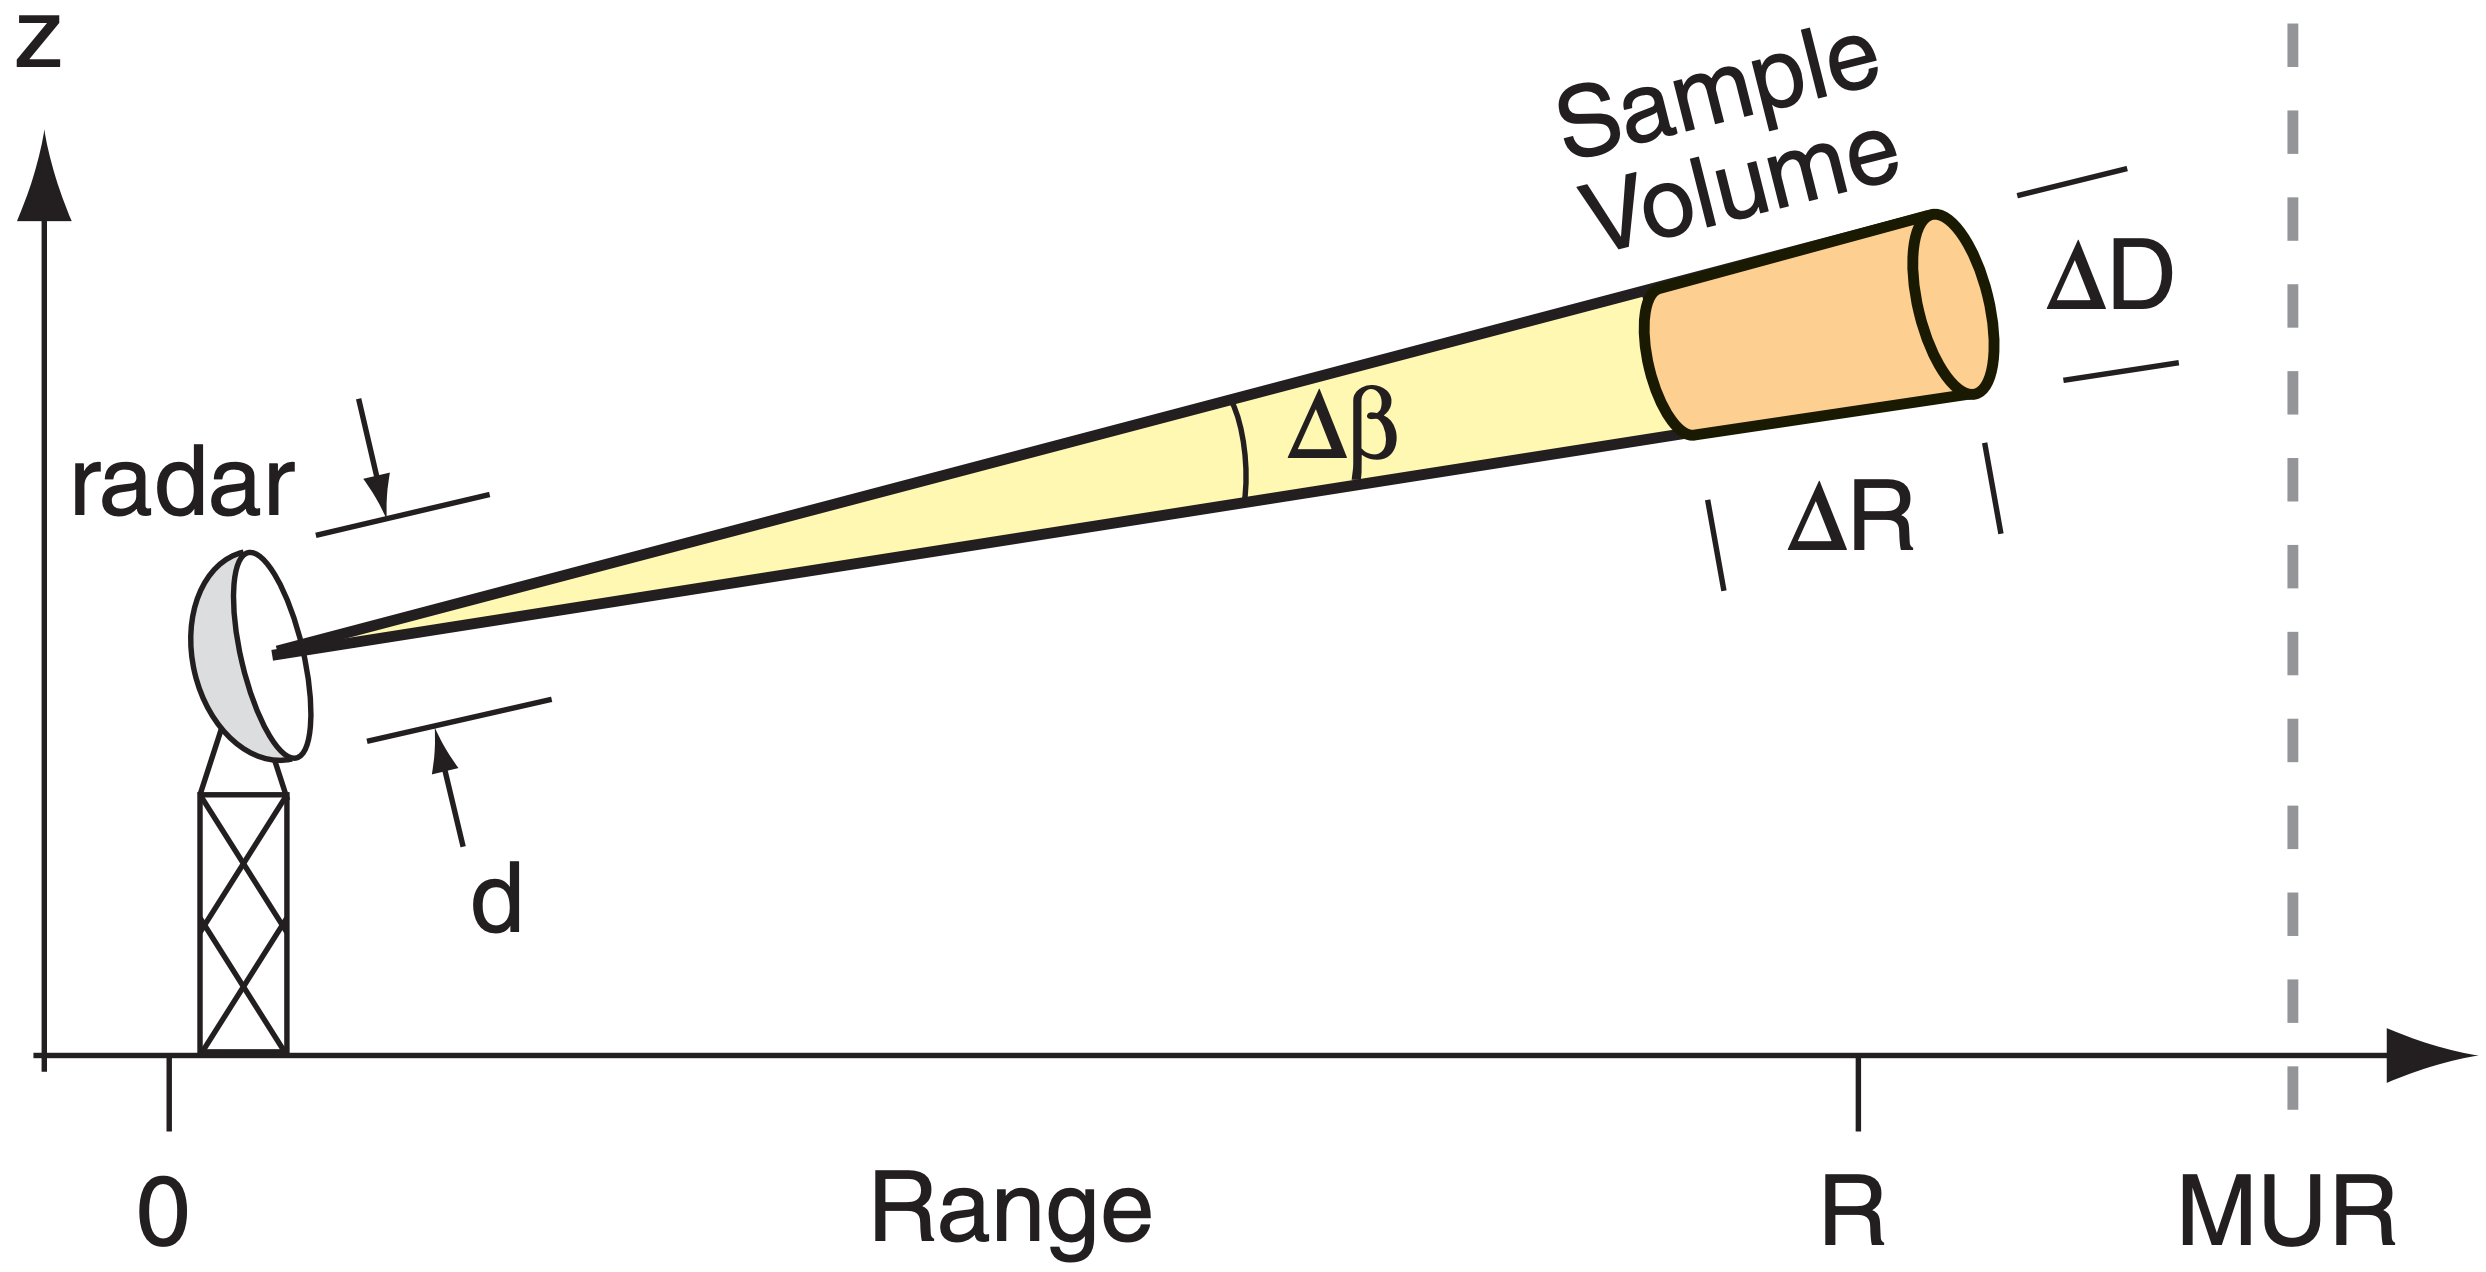
\includegraphics[width=1\linewidth]{Images/radar_concept.png}
    \vspace{2cm}
    \caption{A typical meteorological radar \cite{2022Weather}}
    \label{fig:radar}
\end{figure}

\subsection{Basic terminologies}

\subsubsection{Weather Radar}
% \footnote{Tên tiếng Việt của các thuật ngữ sẽ được căn cứ dựa trên TCVN
% 12636-12 : 2021 \cite{vn_meteor_standard}} Radar thời tiết là một loại cảm
% biến có khả năng phát sóng vô tuyến (bước sóng trong phạm vi từ 250 - 1000 kW)
% \cite{2022Weather}. Để gia tăng cường độ sóng, một chảo antent (attenna dish)
% hình parabol được sử dụng nhằm hội tụ bước sóng. Radar có thể nâng và hạ (tuỳ
% theo yêu cầu) để thu nhập thông tin tại các vị trí chỉ định trong không gian 3
% chiều.

Weather radar, short for weather surveillance radar, is a type of radar system
used to detect and monitor precipitation, as well as other atmospheric phenomena
such as the movement of severe weather systems. It plays a crucial role in
meteorology and helps meteorologists track and forecast weather conditions.
Normally, weather radars are programmed to scan in an azimuth of $360^o$. For
every round, the radar will scan at a different altitude. It usually takes about
four to ten minutes for the radar to complete a full scan.

For PPI representation, the radar will scan the entire azimuth, but only at a
certain altitude. The final result would be similar to a map on a flat surface.
For RHI, in contrast, the radar retains the azimuth but increases in altitude.
The collected result gives viewers more details about the height and sizes of a
meteorologist event.

\begin{figure}[H]
    \centering
    \begin{subfigure}{\textwidth}
        \centering
        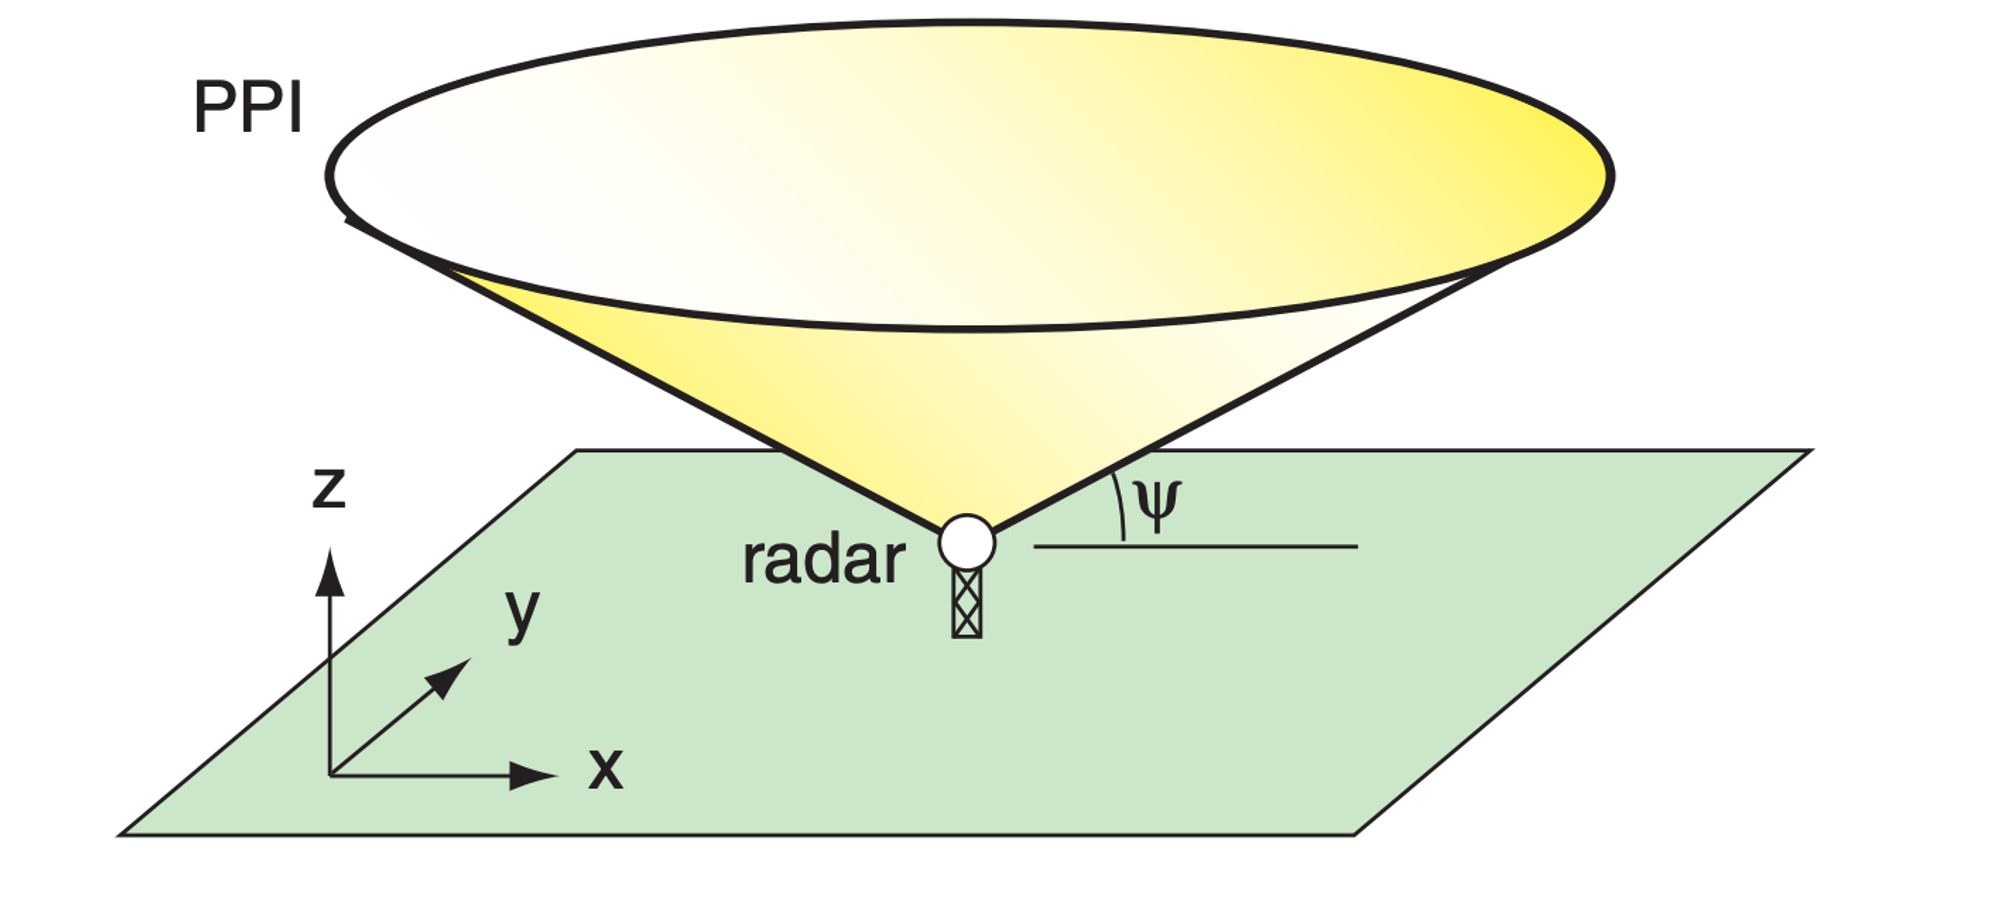
\includegraphics[width=0.85\textwidth]{Images/2.1-ppi.png}
        \caption{Plan-Position Indicator - PPI - \cite{2022Weather}}
        \label{fig:ppi}
    \end{subfigure}

    \begin{subfigure}{\textwidth}
        \centering
        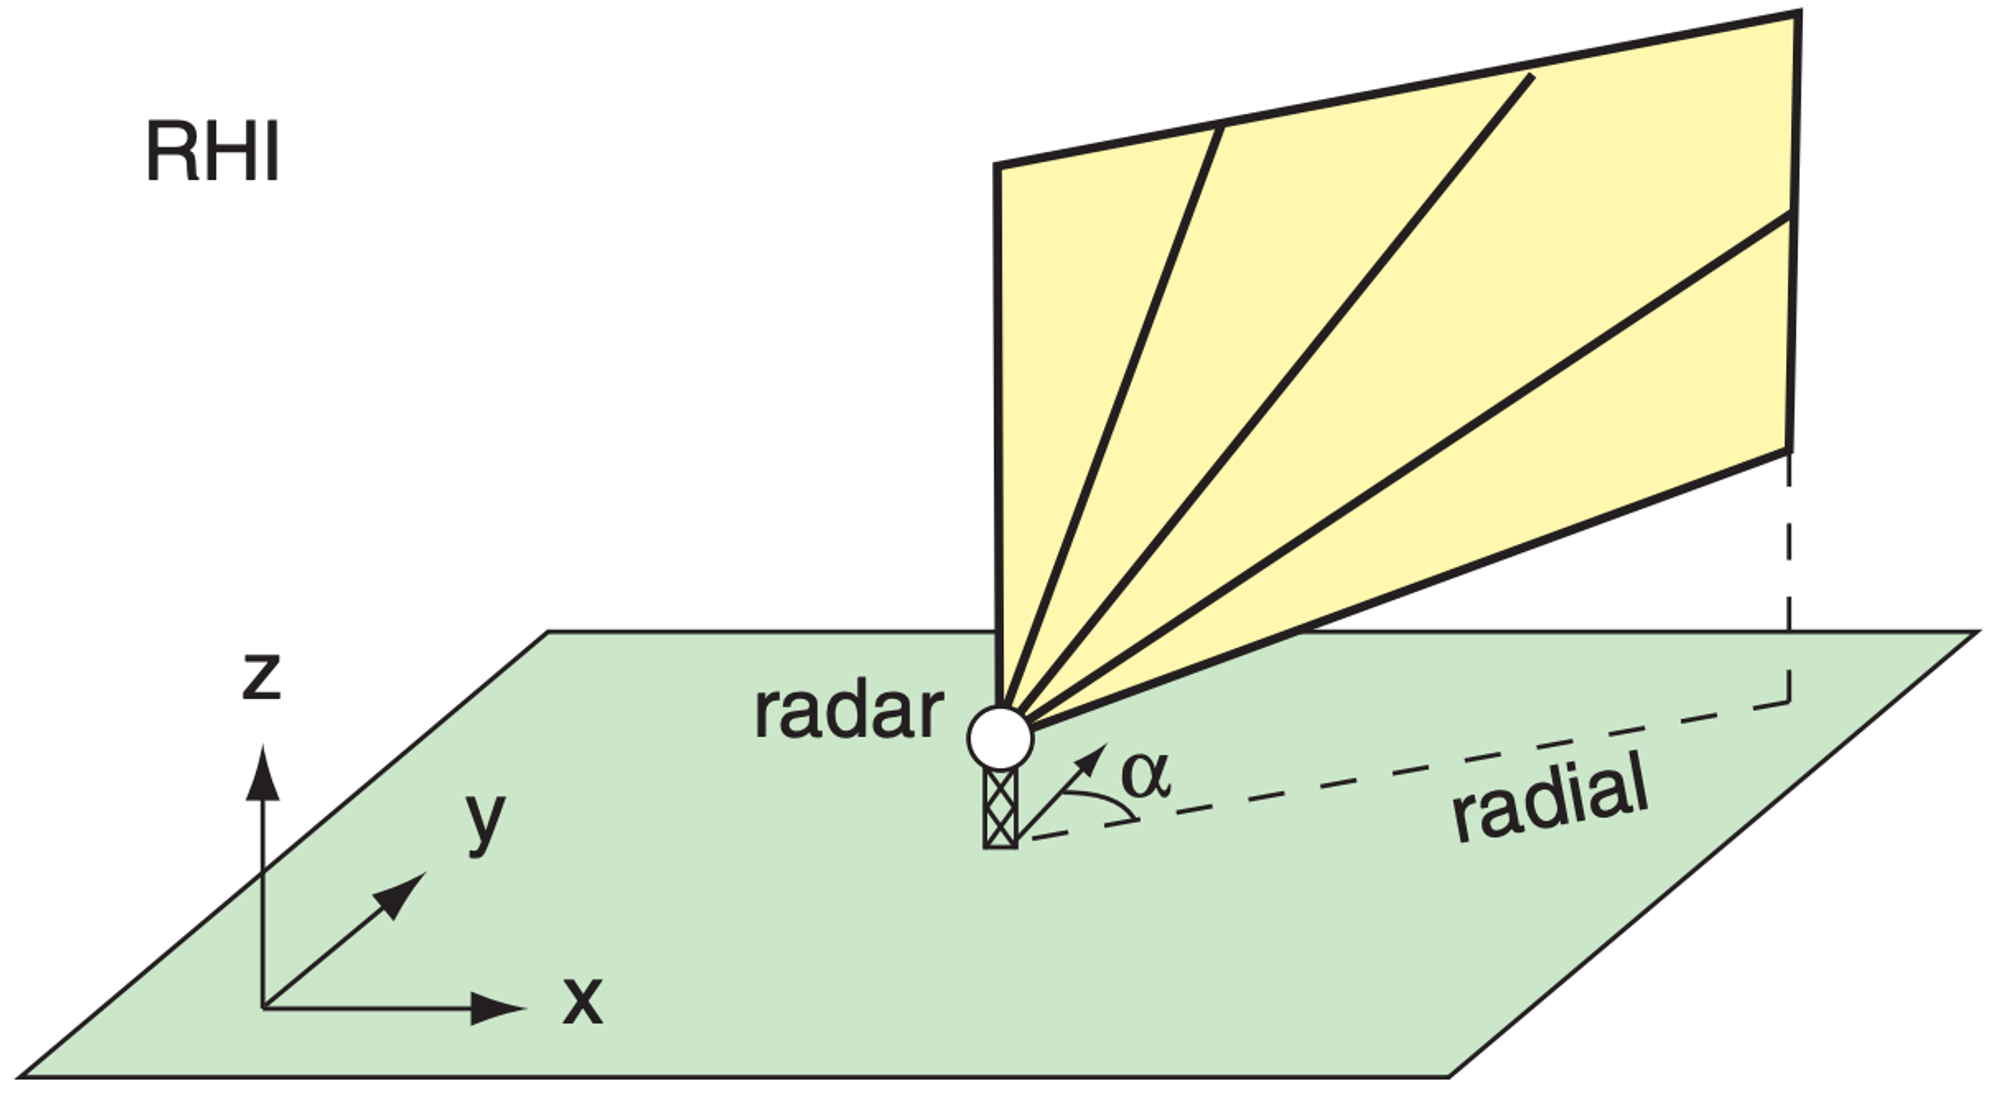
\includegraphics[width=0.85\textwidth]{Images/2.1-rhi.png}
        \caption{Range Height Indicator - \cite{2022Weather}}
        \label{fig:rhi}
    \end{subfigure}

\end{figure}



\begin{figure}[H]
    \centering
    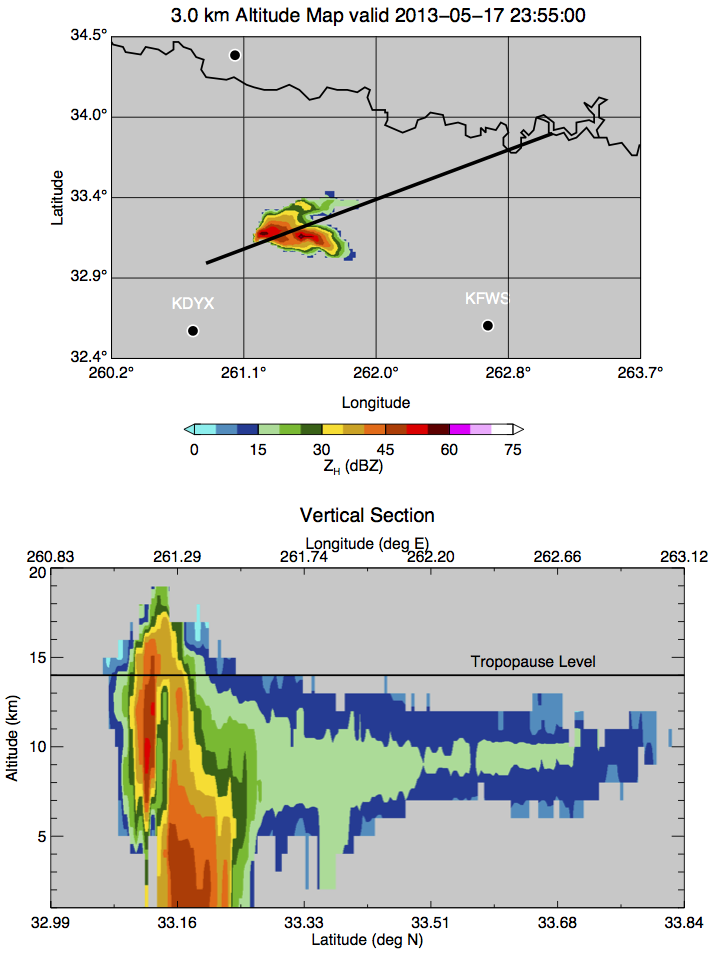
\includegraphics[width=\linewidth]{Images/2.1-ppi-and-rhi.png}
    \caption{Comparing the result between PPI and RHI -
    \cite{stackexchange-ppi-rhi}}
    \label{fig:ppi-and-rhi}
\end{figure}

\subsubsection{Radar equation and Reflectivity}
At a certain point in time, weather radar will emit a short pulse of radio wave
($\Delta t = 0.5 - 10 \mu s$). Depending on the density of free molecules in the
air (water vapor, smoke, ...), the energy of this wavelength will be partially
absorbed. The wavelength intensity that the radar receives will be less than the
intensity of the original wave. This ratio is expressed through \textbf{The
radar equation} \cite{2022Weather}:

\[
    \left[ \frac{P_R}{P_T} \right]=\left[ b \right]\cdot\left[ \frac{|K|}{L_a} \right]^2\cdot\left[ \frac{R_1}{R} \right]^2\cdot\left[ \frac{Z}{Z_1} \right]
\]
\vspace{0.5cm}

Which, the variables of the equation include:
\begin{itemize}
    \item $|K|$ unitless:
          \begin{itemize}
              \item $|K|^2 \approx 0.93$ for droplets
              \item $|K|^2 \approx 0.208$ for ice crystal
          \end{itemize}
    \item $R (\text{km})$: distance from the radar to the target
    \item $R_1 = \sqrt{Z_1 \cdot c \cdot \Delta t / \lambda^2}$: ratio of
    distance
    \item $Z$: Radar's reflectivity
    \item $Z_1 = 1 \text{ mm}^6 \text{ m}^{-3}$: Radar's unit reflectivity
\end{itemize}

From the radar equation, we can derive the formula for reflectivity:
\vspace{0.5cm}
\[
    \text{dBZ} = 10\left[ \log\left( \frac{P_R}{P_T} \right) + 2 \log\left( \frac{R}{R_1} \right) - 2\log\left| \frac{K}{L_a} \right| - \log\left( b \right) \right]
\]

Meteorologists are usually interested in this number because it is proportional
to the amount of precipitation.

\begin{table}[h]
    \centering
    \begin{tabular}{|c|l|}
        \hline
        Value (dBZ) & Weather               \\
        \hline
        -28         & Haze                  \\
        -12         & Clear air             \\
        25 - 30     & Dry snow / light rain \\
        40 - 50     & Heavy rain            \\
        75          & Giant hail            \\
        \hline
    \end{tabular}
    \vspace{1em}
    \caption{ Relation between reflectivity and precipitation -
    \citet{2022Weather}}
\end{table}

\begin{figure}[H]
    \centering
    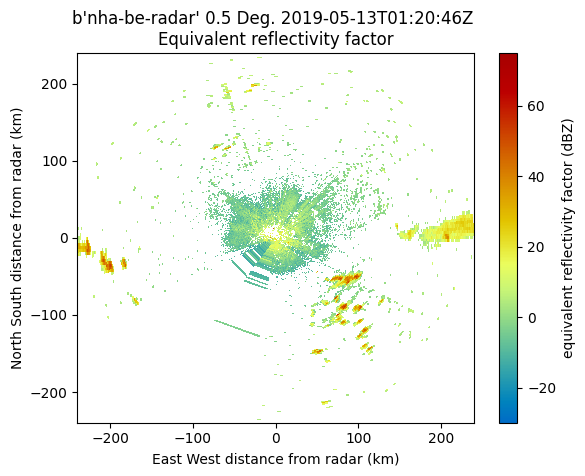
\includegraphics[width=0.75\textwidth]{Images/2.1-reflectivity_nhabe.png}
    \vspace{1em}
    \caption{Reflectivity from Nha Be radar}
    \label{fig:reflectivity-nhabe}
\end{figure}

\subsubsection{Radial velocity}

\begin{figure}[H]
    \centering
    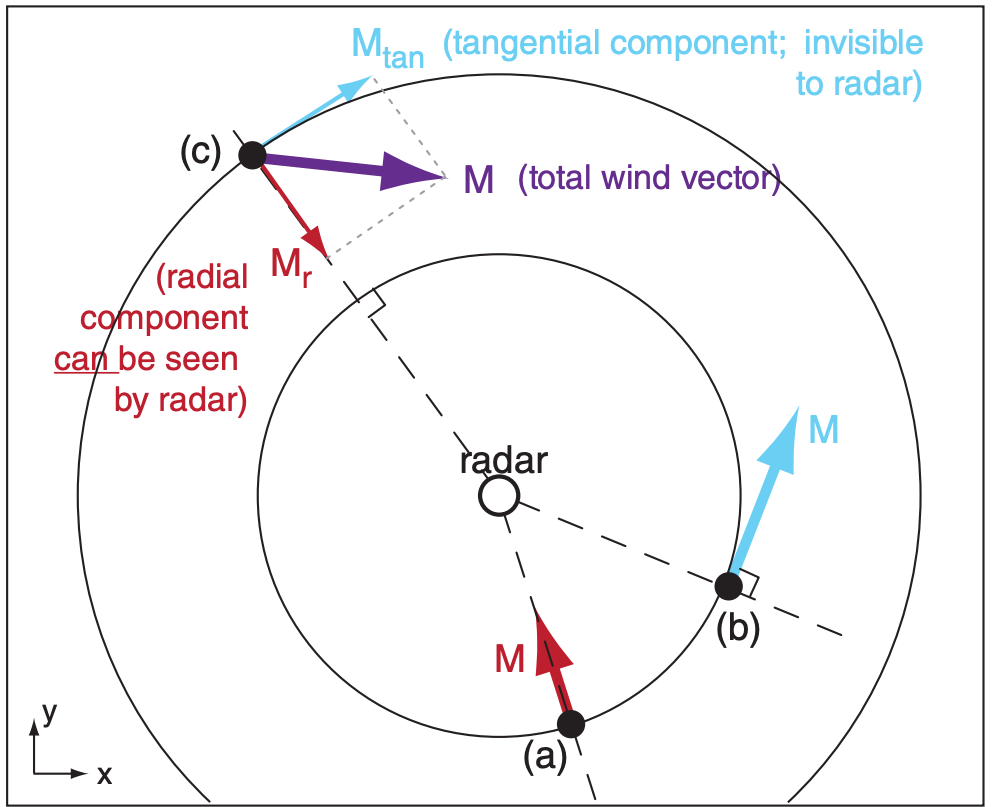
\includegraphics[width=.55\textwidth]{Images/2.1-radial-velocity.png}
    \vspace{2em}
    \caption{Illustration for the velocity situations that a Doppler radar can
    observe. (a) When the wind direction at point M coincides with the radius of
    the circle centered at the radar, the radar can determine the velocity at
    this point. (b) When the wind direction is tangent to the circle, the radar
    cannot determine the velocity. (c) Analyzing the wind direction at M into
    two perpendicular velocities, the radar can only determine the velocity
    vector along $M_r$.  - \citet{2022Weather}}
    \label{fig:radial-velocity}
\end{figure}

When the radio waves from these Doppler radars propagate to the molecules in the
air, the displacement of these particles causes a phase shift between the
transmitted and received signals. Radars rely on this information to calculate
the wind velocity at various points in space.

\subsection{Radar Products}

\subsubsection{Echo Top Height (ETH)}
An echo top, in radar meteorology, signifies the highest altitude at which
precipitation particles are detected. Essentially, it helps us pinpoint the
maximum elevation angle where the intensity of precipitation, quantified by
reflectivity, surpasses a predetermined threshold. This information is crucial
for understanding the vertical extent of precipitation systems and their
potential impact. 

\subsubsubsection*{\underline {Overview}}

The modified ETH algorithm, developed by Lakshmanan et al. (2013) [Lakshmanan et
al. (2013):
https://journals.ametsoc.org/view/journals/wefo/28/2/waf-d-12-00084\_1.xml], can
be applied to a NEXRAD PPI volume scan by following these steps:
\begin{enumerate}
    \item \textbf{Finding Echo Top Height:} \\
    Locate the maximum elevation angle, denoted by $\theta_{b}$, where the
reflectivity, $Z_{b}$, surpasses a predefined echo-top reflectivity threshold,
$Z_T$ (e.g., 0 dBZ, 18 dBZ). If $\theta_{b}$ is not the highest elevation scan
available in the volume, obtain the reflectivity value, $Z_{a}$, at the
subsequent higher elevation angle, $\theta_{a}$. Employ the following equation
to calculate the echo-top height, $\theta_T$:

$$\theta_T = \frac{(Z_T - Z_a) (\theta_b - \theta_a)}{Z_b - Z_a} + \theta_b$$

    \item \textbf{Handling Highest Elevation Scan:}\\
    If $\theta_{b}$ coincides with the highest elevation scan accessible, set
    $\theta_{T} = \theta_{b} + \beta/2$, where $\beta$ represents the half-power
    beamwidth. This scenario arises when:
    \begin{itemize}
        \item Far from the radar: Higher elevation scans possess shorter ranges
    compared to a baseline "surveillance" scan.
        \item Very close to the radar: The highest elevation scan fails to
    capture the cloud's peak.
    \end{itemize}
    
Under these circumstances, $\theta_{T}$ corresponds to the top of the beam
containing reflectivity greater than or equal to $Z_T$. In essence, the
traditional echo-top computation is adopted when no data exists from higher
elevation scans.

This mathematical formulation can be expressed in LaTeX as:

$$\theta_T = \begin{cases} \frac{(Z_T - Z_a) (\theta_b - \theta_a)}{Z_b - Z_a} +
\theta_b & \text{if } \theta_b \text{ is not highest elevation scan} \\
\theta_b + \frac{\beta}{2} & \text{if } \theta_b \text{ is highest elevation
scan} \end{cases}$$

This equation incorporates a conditional statement to account for the two
scenarios based on the availability of data from higher elevation scans.

\end{enumerate}